\documentclass[prb,preprint]{revtex4-1} 
% The line above defines the type of LaTeX document.
% Note that AJP uses the same style as Phys. Rev. B (prb).

\usepackage{amsmath}  % needed for \tfrac, \bmatrix, etc.
\usepackage{amsfonts} % needed for bold Greek, Fraktur, and blackboard bold
\usepackage{graphicx} % needed for figures
\usepackage{tabularx}
\usepackage{color}
\DeclareMathOperator{\sinc}{sinc}
\begin{document}

\title{Double-Slit Experiment  ---need more exciting title here, relevant to physics that is demonstrated, particularly light as a wave}
% In a long title you can use \\ to force a line break at a certain location.

\author{Yumeng Melody Cao}
\email{mcao@smith.edu} % optional
% If there were a second author at the same address, we would put another 
% \author{} statement here.  Don't combine multiple authors in a single
% \author statement.
\affiliation{Department of Physics, Smith College, Northampton, MA 01063}
% Please provide a full mailing address here.

\author{He Claudia Yun}
\email{hyun@smith.edu}
\affiliation{Department of Physics, Smith College, Northampton, MA 01063}

% See the REVTeX documentation for more examples of author and affiliation lists.

\date{\today}

%____________abstract____________________________________________

\begin{abstract}
%The motivation of this experiment originates from the interference of light waves caused by 
%originated from that, this experiment we use the TWS apparatus with a laser of wavelength 670nm to re-perform Young's Double-Slit Experiment. 

% shown in Fig.\ref{image}
When a coherent laser beam passes through two narrow slits, these two light beams of a constant phase difference will diffract from each slit and spread out passing through each other. This leads to constructive and destructive interference that can be detected on a screen at some distance from the slits. This phenomenon shows the wave nature of light. 
%This experiment, also known as the Young$^\prime$s double-slit experiment, 
Originally done by Young back in 1800, the double-slit experiment was reproduced in this lab with the use of the TWS apparatus with a laser of 670nm in wavelength. The monochromatic light beam was sent from one end of a u-channel through a double-slit to create an interference pattern. The photodiode at the other end measures the light intensity and by moving a slit across the detector, variations in light intensity can be used to infer the interference pattern. 
%The results and the plots in the experiment successfully demonstrated the wave nature of light. 
The observed interference pattern is fitted using Fraunhofer model, which describes far-field diffraction. The amplitude of the double-slit pattern was observed to be the modulated by the single slit diffraction pattern. Reduced $\chi^2$ of the double-slit fit curve is 0.827 and that of the single-slit fit curve is 1.57, both indicating that the data are consistent with the model within our estimate of uncertainty.

%{\color{blue} comments on abstract
%\begin{enumerate}
%\item don't include references to figures (or figures) in abstract! Abstract needs to be able to ``stand alone.''  You should move Figure 1 to the introduction. 
%\item first statement isn't always true. The two beams of light need to have come from the same source, and be coherent. That is, there needs to be a definite and constant phase difference between the two (even if that difference is zero, and they are therefore in phase with each other). 
%\item first sentence is also misleading. It reads as is you are saying that the projection on the screen causes the interference, which certainly isn't true. The screen is how the variation in light intensity due to wave interference is detected, not how it is caused.  Physically, it is because the waves diffracting from each slit spread out, passing through each other. That leads to constructive and destructive interference (peak + peak = bigger peak, valley + valley = deeper valley, peak + valley = flat (null) node).  You should include a sentence or two discussing this, so that the reader can understand that the detected interference pattern provides evidence for the wave nature of light. 
%\item the photodiode measures light intensity, and hence can be used to measure variations in light intensity as a function of some other variable. It doesn't detect interference patterns directly. you had to select different parts of that pattern (by moving a slit across the detector) to detect the interference pattern. 
%\end{enumerate}
%}

\end{abstract}

\begin{figure}[b]
\centering
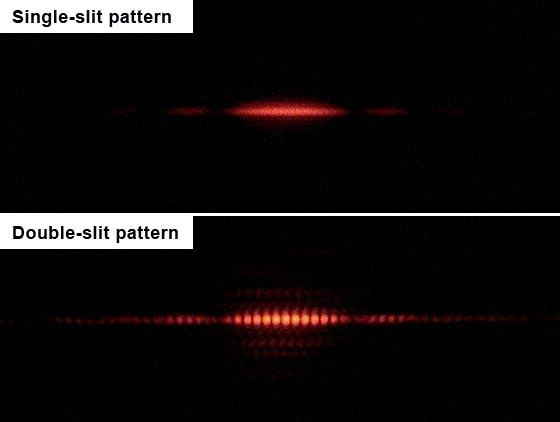
\includegraphics[width=3in]{image1.jpg}
\caption{Single and double-slit interference patterns \cite{wik}.}
%
\includegraphics[width=1in]{white.png}
\label{image}
\end{figure}

\maketitle 

%____________Introduction____________________________________________
\section{Introduction}
The double-slit experiment --- also known as the Young$^\prime$s experiment --- explores the wave-like nature of light. It is important in this experiment that the two sources of light are coherent and have a constant phase difference.
%\textcolor{blue}{don't have to be same phase, but they do need to have a constant phase difference. Can still get an interference pattern if phase difference is $Pi/2$ instead of zero --- the pattern will just have all the double slit interference maxima and minima reversed!}. 
Back in 1801, Thomas Young had difficulty with using common light sources, such as candles and lanterns, to be served as coherent sources of light. Thus instead, Young performed the experiment by filtering sunlight through a pinhole in a window shutter split by a piece of card and projecting it horizontally across the room. Light waves from either side of the card coming through the pinhole can be thus considered coherent sources and the interference pattern was then projected onto a screen. (See Fig. \ref{interference})

\begin{figure}[h]
\centering
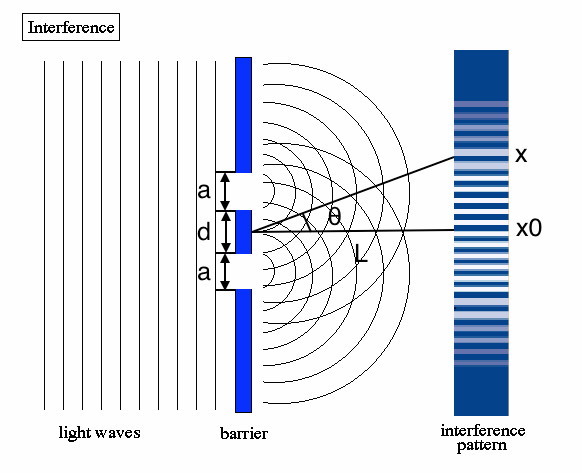
\includegraphics[width=5in]{interference.png}
\caption{Calculate angle from position \cite{interference}. L being the distance between the slits and the photo diode($\approx50cm$); a being the slit width; d being the slit separation; x0 being the location reading on the detector slit micrometer at the central maximum; x being the location reading on the detector slit micrometer at different values to obtain the intensity at that distance from the central maximum; $\theta$ being the angle between the central maximum and value of x. How x is calculated is included in the discussion section. (Eq. \ref{theta}); }
\label{interference}
\end{figure}

First looking at the double slit experiment, to create the curve of best fit, the Fraunhofer equation is applied to the double-slit intensity: 

\begin{equation}
I=I_0 \sinc^2{\left(\frac{\pi a}{\lambda}\sin{\theta}\right)}  \cos^2{\left(\frac{\pi d}{\lambda} \sin \theta\right)}
\label{eq1}
\end{equation}
%\textcolor{red}{where, since not everyone who is a likely reader of this report would know what sinc is, you should define }
\begin{equation*}
\sinc(\alpha) \equiv \frac{\sin(\alpha)}{\alpha}
\end{equation*}

The Fraunhofer conditions can be applied once again to create  the curve of best fit for the single-slit experiment: 
\begin{equation}
I=I_0 \sinc^2 \left(\frac{\pi a}{\lambda} \sin\theta \right)
\label{eq2}
\end{equation}

%\textcolor{magenta}{This would be a good place to derive equations (1) and (2), since you introduce them without explanation later in your results and analysis section. Include text and a figure that defines your variables.}

%\textcolor{blue}{I'm not sure what the point of the equation above is, since it isn't the equation you use later, and is in fact just a small angle approximation replacing $\sin(\theta)$ with $\theta$. If you think it is helpful, however, then you need to define what the variables mean!  How will anyone know what $m$ or $d$ are?  YOu would also need a figure. It might be similar to your Figure (2) if you add lines indicating the meanings of $L$, $\theta$, and $y$ etc, or it might be similar to Figure (5), although that figure doesn't indicate what $m$ is and uses different variables from those in the above equation. For example, it has $D$ equal to what your formula calls $L$ instead of what your formula calls $d$.  } 

%____________Experiment____________________________________________
\section{Experiment}

Today, we can do the experiment by using the TeachSpin's Two-Slit interference (TWS) apparatus that includes a monochromatic laser beam at one end (with a wavelength of 670 nm) passing through a double slit all encapsulated in a tightly sealed \textcolor{blue}{does this mean ``light-tight''?} u-channel. Adjusting the micrometer attached to the detector-slit allows you to gather information regarding the interference pattern that is projected to a photodiode at the other end of the u-channel. \textcolor{blue}{what detector slit? It needs defining. A bit wordy possibility --- you can do better --- might be `a slit that can be moved laterally across the detector to pick out individual maxima and minima in the interference pattern ...'}


In this experiment, the apparatus is set up as shown in Fig. \ref{dia}. After precise alignment of the laser, the double-slit, the slit-blocker, and the detector-slit, the photodiode is connected to a multimeter which is ultimately connected to the computer. LabView is used to collect data first for the double-slit experiment and for the single-slit experiment. \\

\begin{figure}[h!]
\centering
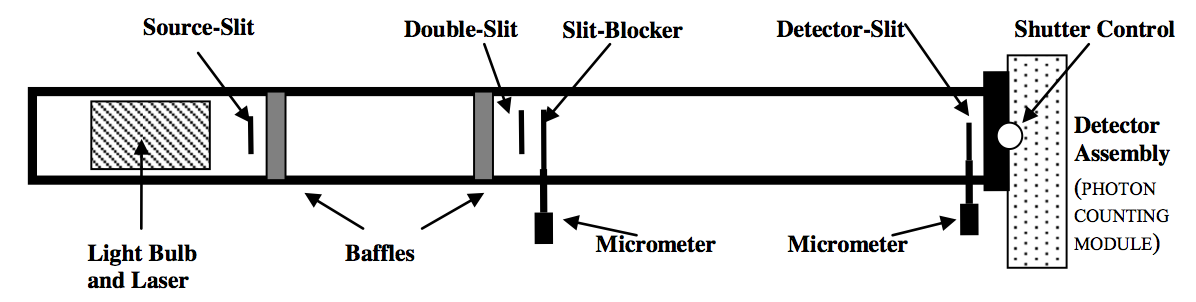
\includegraphics[width=7in]{dia}
\caption{Schematic of TWS apparatus - not to scale \cite{dia}.}
\label{dia}
\end{figure}
All parts are carefully aligned \textcolor{blue}{how is this done? did you follow a particular instruction sheet? what is the criteria for alignment?} and key positions of the slit-blocker are recorded, so that light from one or two slits could be blocked and form \textcolor{red}{both} double-slit and single-slit interference patterns. \textcolor{red}{this is misleading. I think you are using the slit blocker to} select \textcolor{red}{between single-slit and double-slit diffraction experiments. Depending on the experiment chosen, you then either see a single-slit interference pattern dependent on the ratio $a/\lambda$ of the slit width $a$ to the light wavelength $\lambda$ or a double-slit pattern    with a bright-fringe to bright-fringe spacing dependent on the ratio $d/\lambda$ of the slit spacing $d$ to the light wavelength $\lambda$, modulated by a single-slit pattern due to the finite widths of the two slits } The shutter at the end of the U-channel was kept closed, because only the photodiode on the surface of the shutter is used. \textcolor{blue}{what does the shutter block? what would be exposed to light if it were open?} After the preparation work, the double-slit experiment is first performed. A double-slit \textcolor{red}{of} \textcolor{blue}{with?} slit width approximately 0.1 mm and slit separation 0.406 mm \textcolor{red}{is used}. \textcolor{magenta}{don't yet get a choice of slit separations? if so, ``was chosen'' or ``was used'' would be  better choices than ``is used.''}  \\

The slit-blocker is set at the position where light from both slits are allowed to pass, and the detector-slit is set at the position of the central maximum. The photodiode outputs a voltage that is proportional to the intensity of the laser beam. \textcolor{red}{The laser beam intensity is constant. Don't you mean something related to the interference pattern that actually varies?}\\ 

By changing the position of the detector-slit, intensity of the laser light is recorded by LabView as a function of location. \textcolor{red}{same comment: not measuring intensity of laser light, measuring intensity of interference pattern due to constructive and destructive interference of the light waves diffracting from each slit (or slit edge). Don't say exactly that -- I'm being wordy and overprecise here}  Then the experiment is repeated for single-slit when the slit-blocker blocks light from one of the two slits. \\
%____________Results____________________________________________
\section{Results}

\begin{figure}[h]
\centering
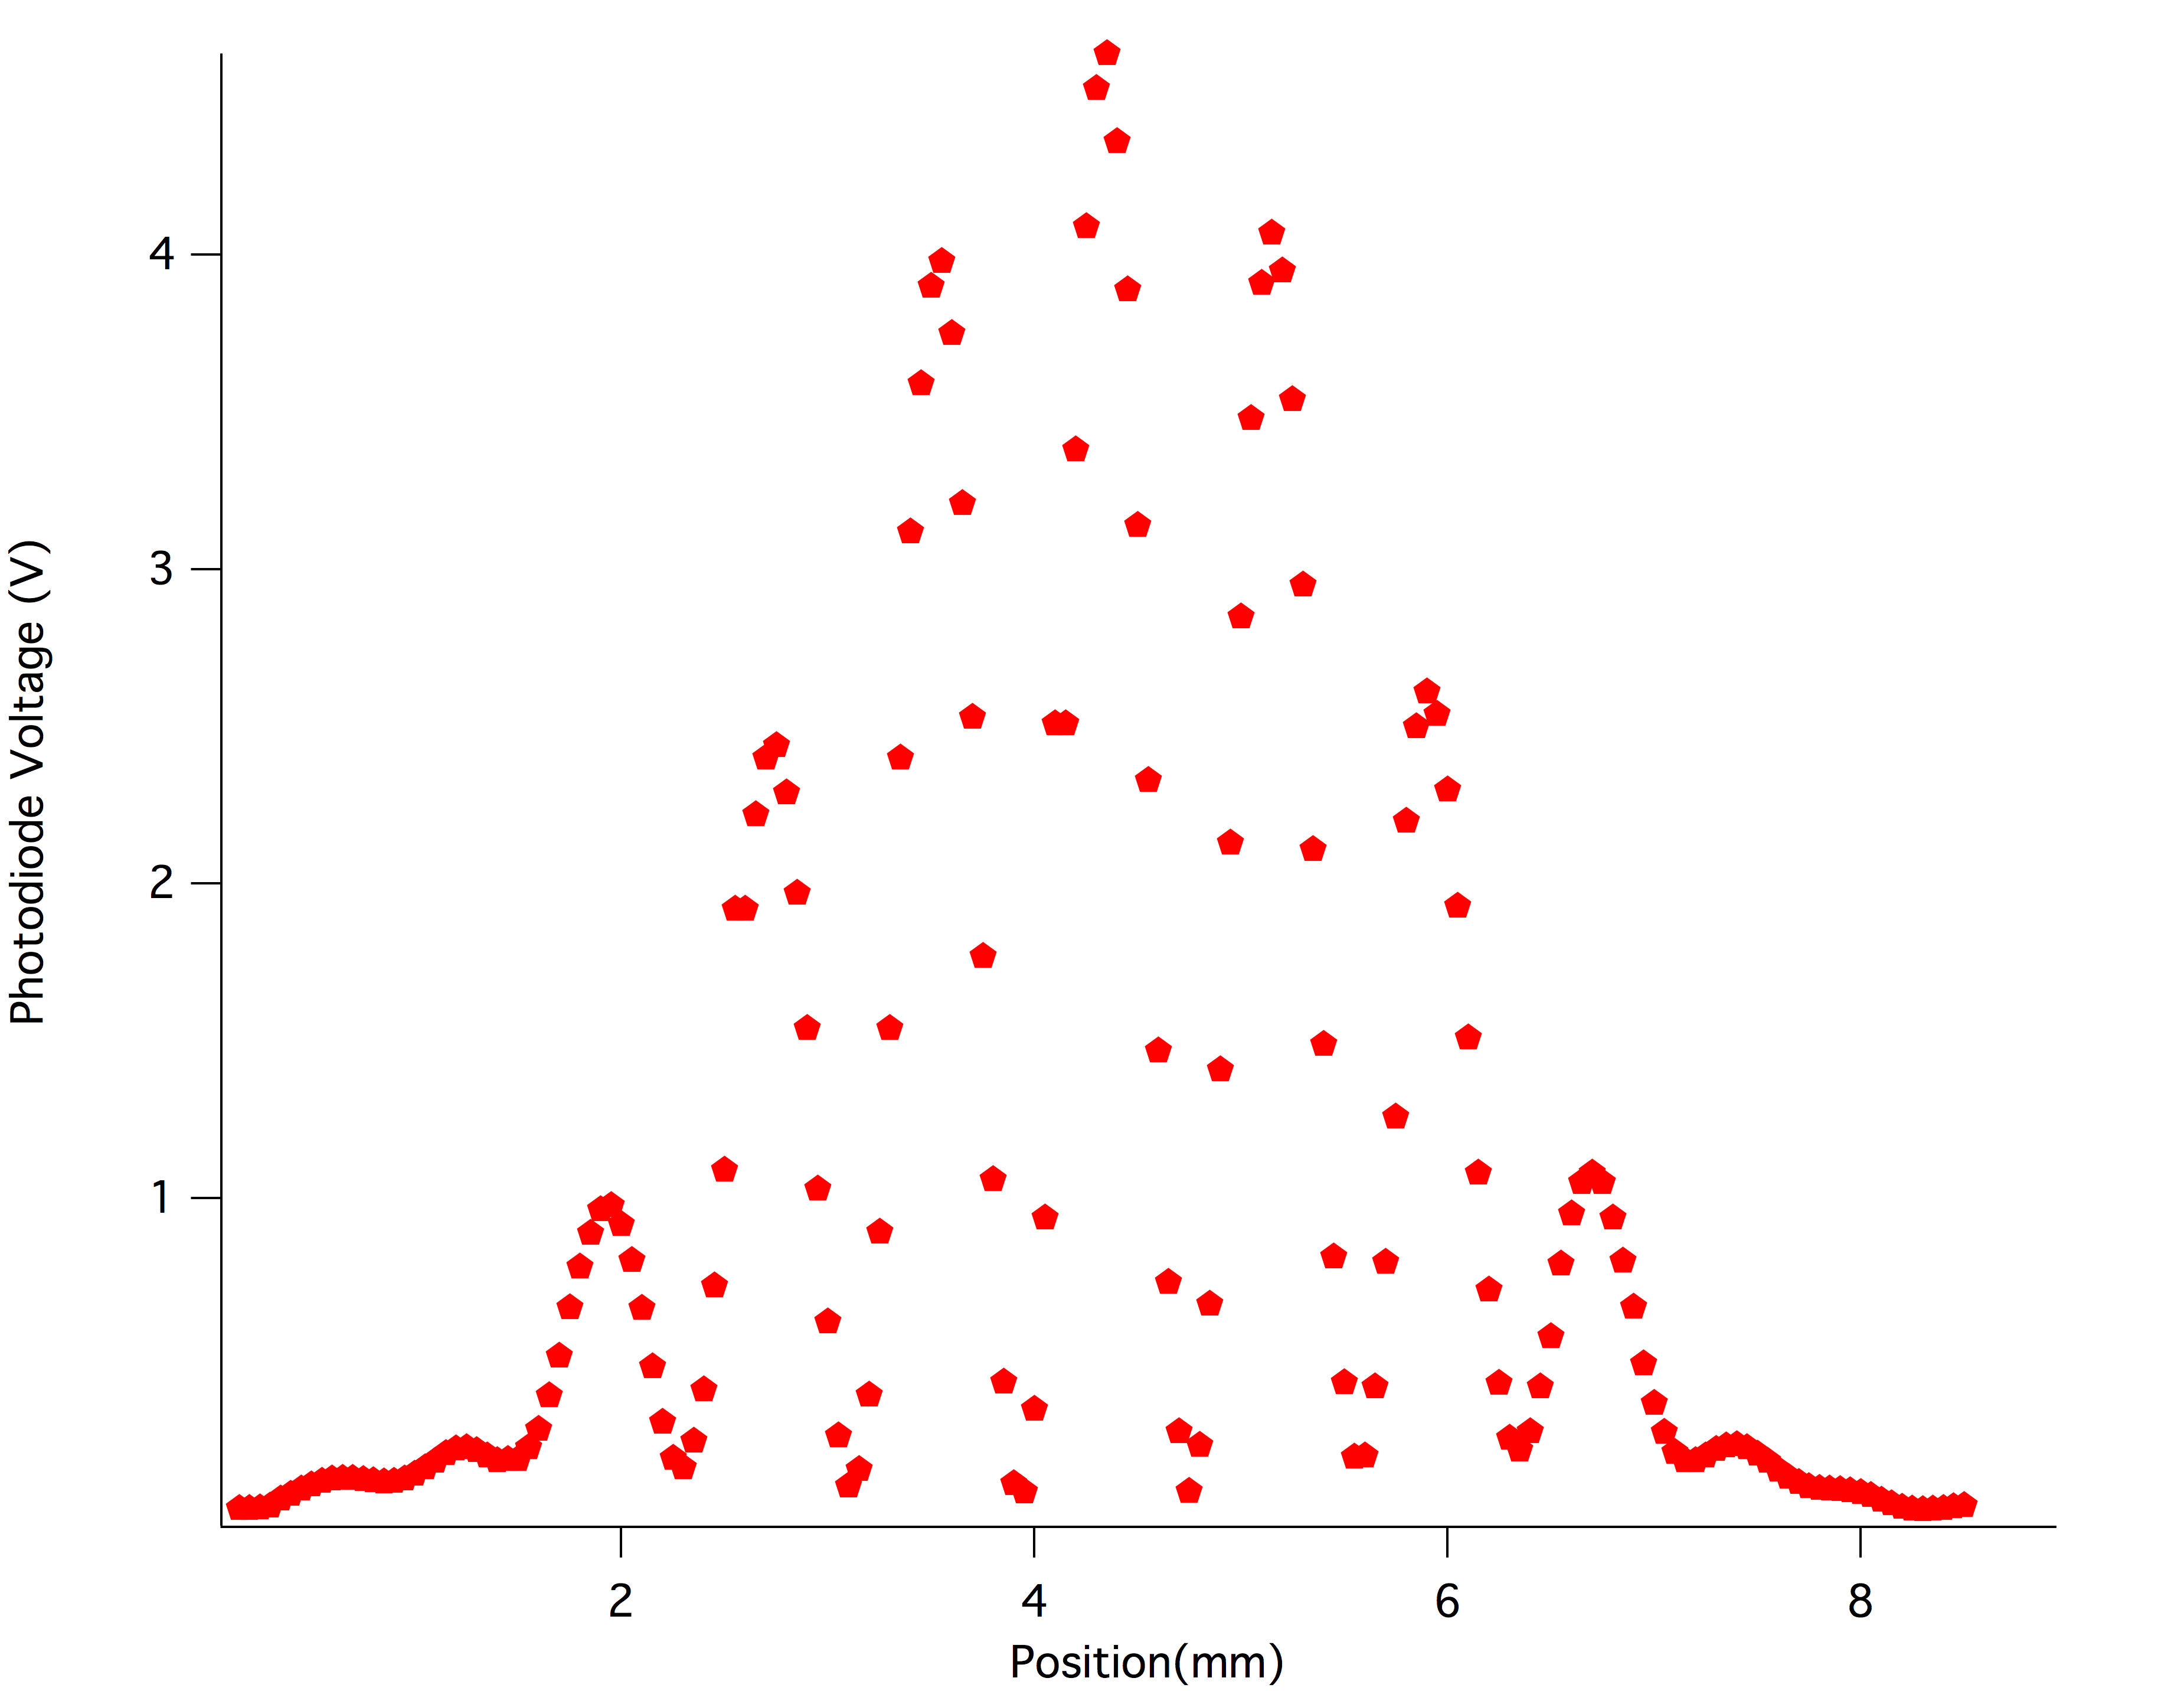
\includegraphics[width=3.2in]{doubleres.png}
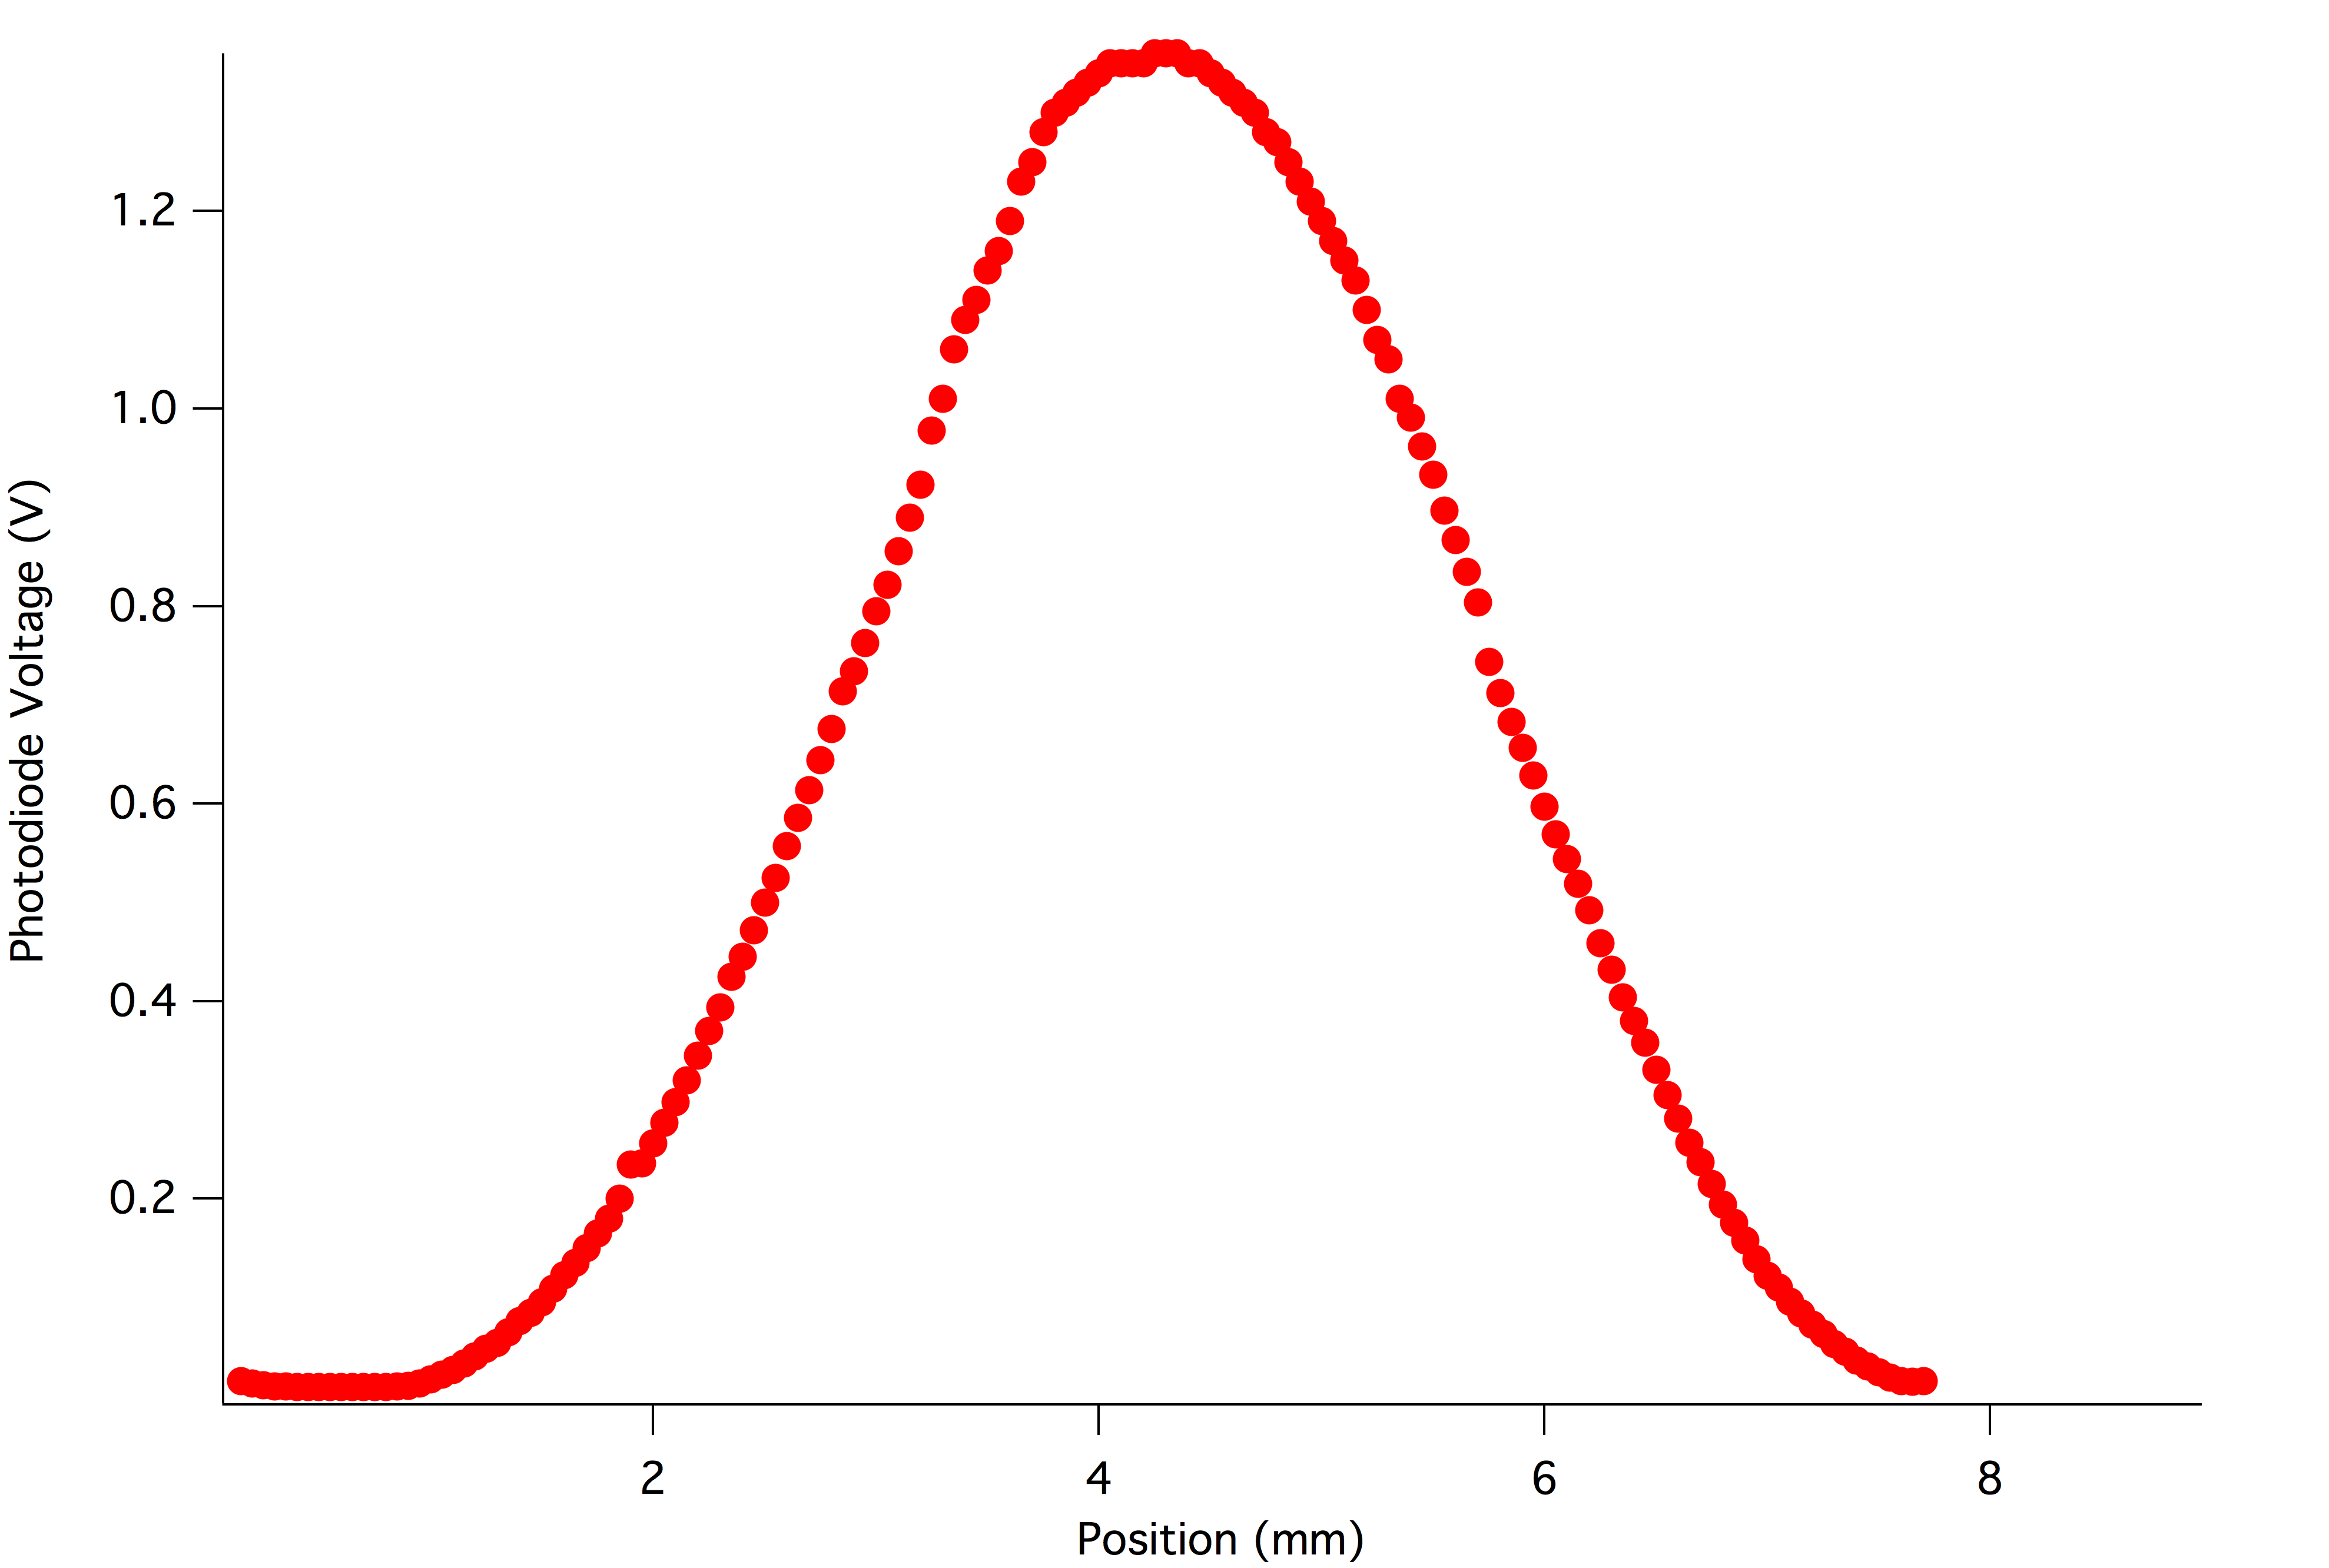
\includegraphics[width=3.2in]{singleres.png}
\caption{Recorded data for double (left) and single-slit (right) interference experiments.}
\label{ds}
\end{figure}

\newpage

The recorded raw data for the double and single-slit experiments are shown in Fig.\ref{ds}. 

Using plotting tools and a non-linear least squares curve fitting routing in Igor Pro while applying Eq. \ref{eq1}, we can obtain the plot shown below in Fig. \ref{double}. Calculation of the error bars will be included in the discussion section.

\begin{figure}[h]
\centering
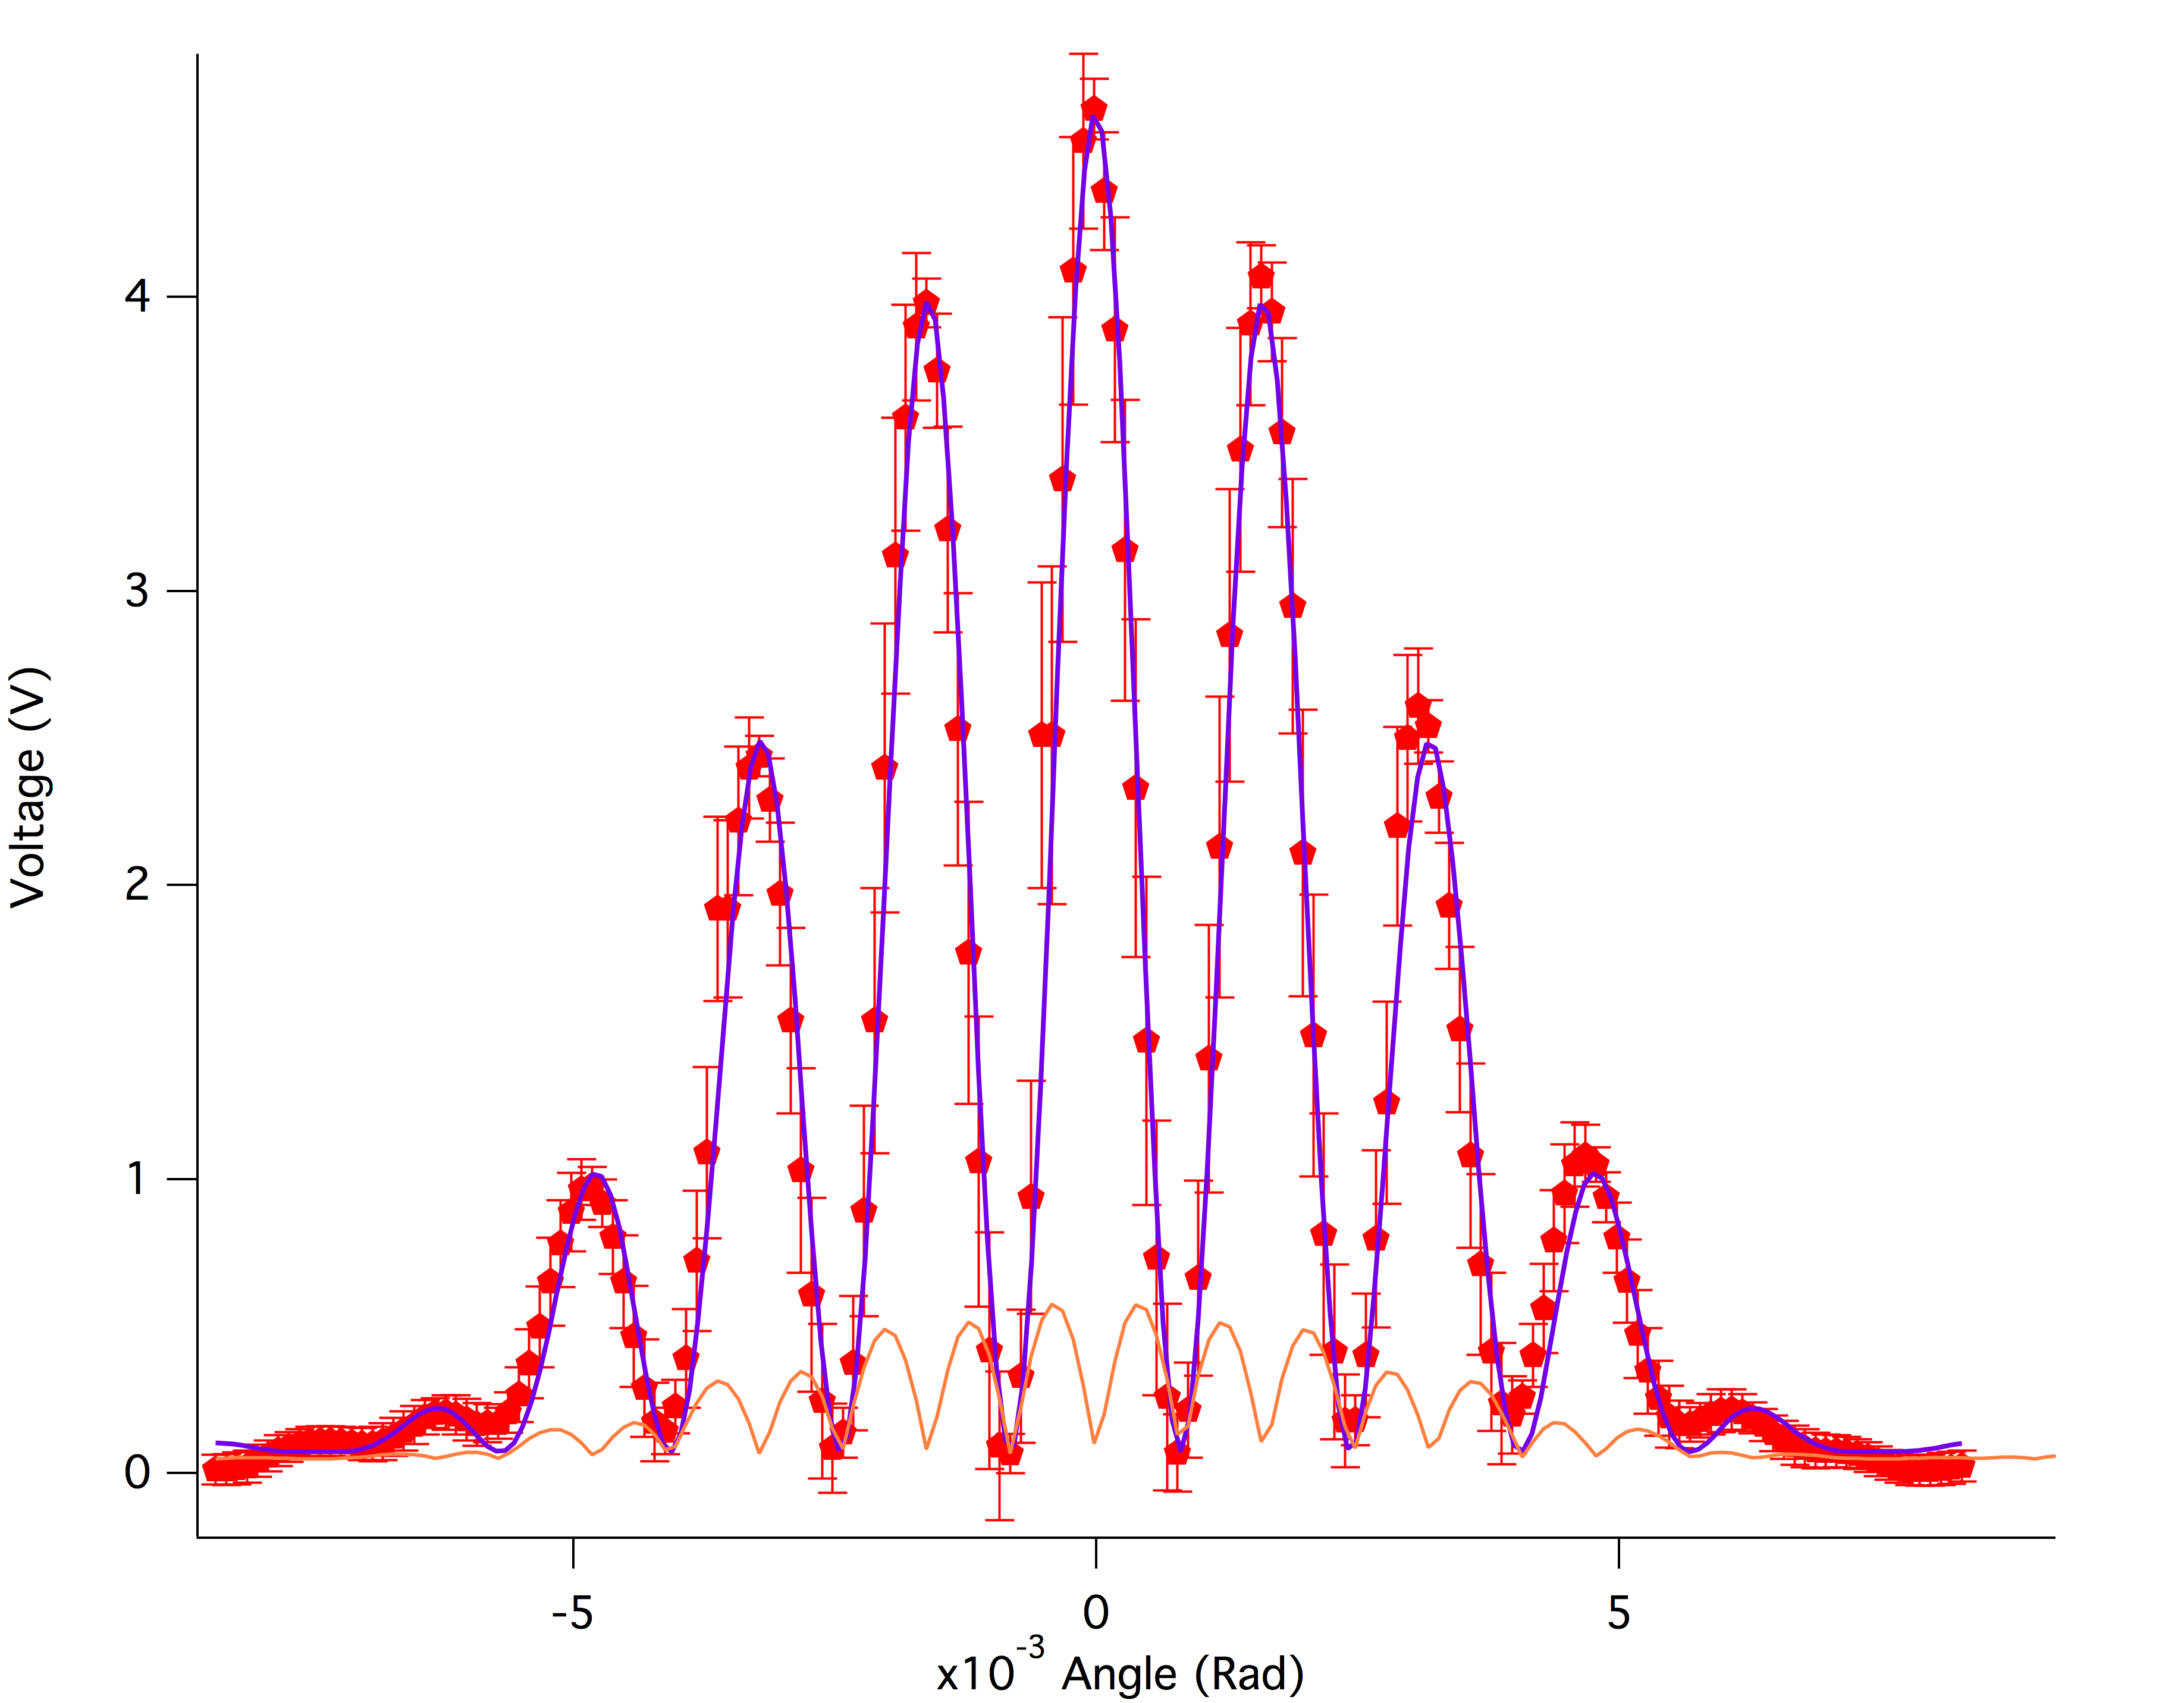
\includegraphics[width=7in]{double.png}
\caption{Plot of raw data, error bars and fit curve of the double-slit experiment. The y-axis is the voltage the photodiode outputs which is proportional to the intensity of light shining on it, and the x-axis is the angle away from the central maximum (Fig. \ref{interference}). The curve at the bottom of the graph shows the size of error as a function of angle.}
\label{double}
\end{figure}


\begin{table}[h]
\centering
\caption{Double-slit data. \textcolor{red}{the variables a and d are missing from Figure 5, and in Figure 5 D is mislabeled as the length L from the slits to the detector instead of the distance d between the slits}}
\begin{ruledtabular}
\begin{tabular}{ l c c c}
Name & Symbol & Value & Uncertainties($\pm$)\\
\hline
Slit width & a & 88.3 $\mu m$ & 0.4 $\mu m$\\
Slit separation & d & 426.89 $\mu m$ & 0.07 $\mu m$\\
Wavelength & $\lambda$ & 0.67 nm & N/A \\
Max voltage & $V_0$ & 4.55 V & 0.07 V\\
Voltage offset & $V_{offset}$ & 0.073 V & 0.008 V\\
Theta offset &$ \theta_{offset}$ & 1E-05 rad & 8E-06 rad \\
\hline
Chi Squared & $X^2$ & 0.827068&
\end{tabular}
\end{ruledtabular}
\label{data}
\end{table}

\newpage

The Fraunhofer conditions can be applied once again to create  the curve of best fit for the single-slit experiment: 

\begin{figure}[h]
\centering
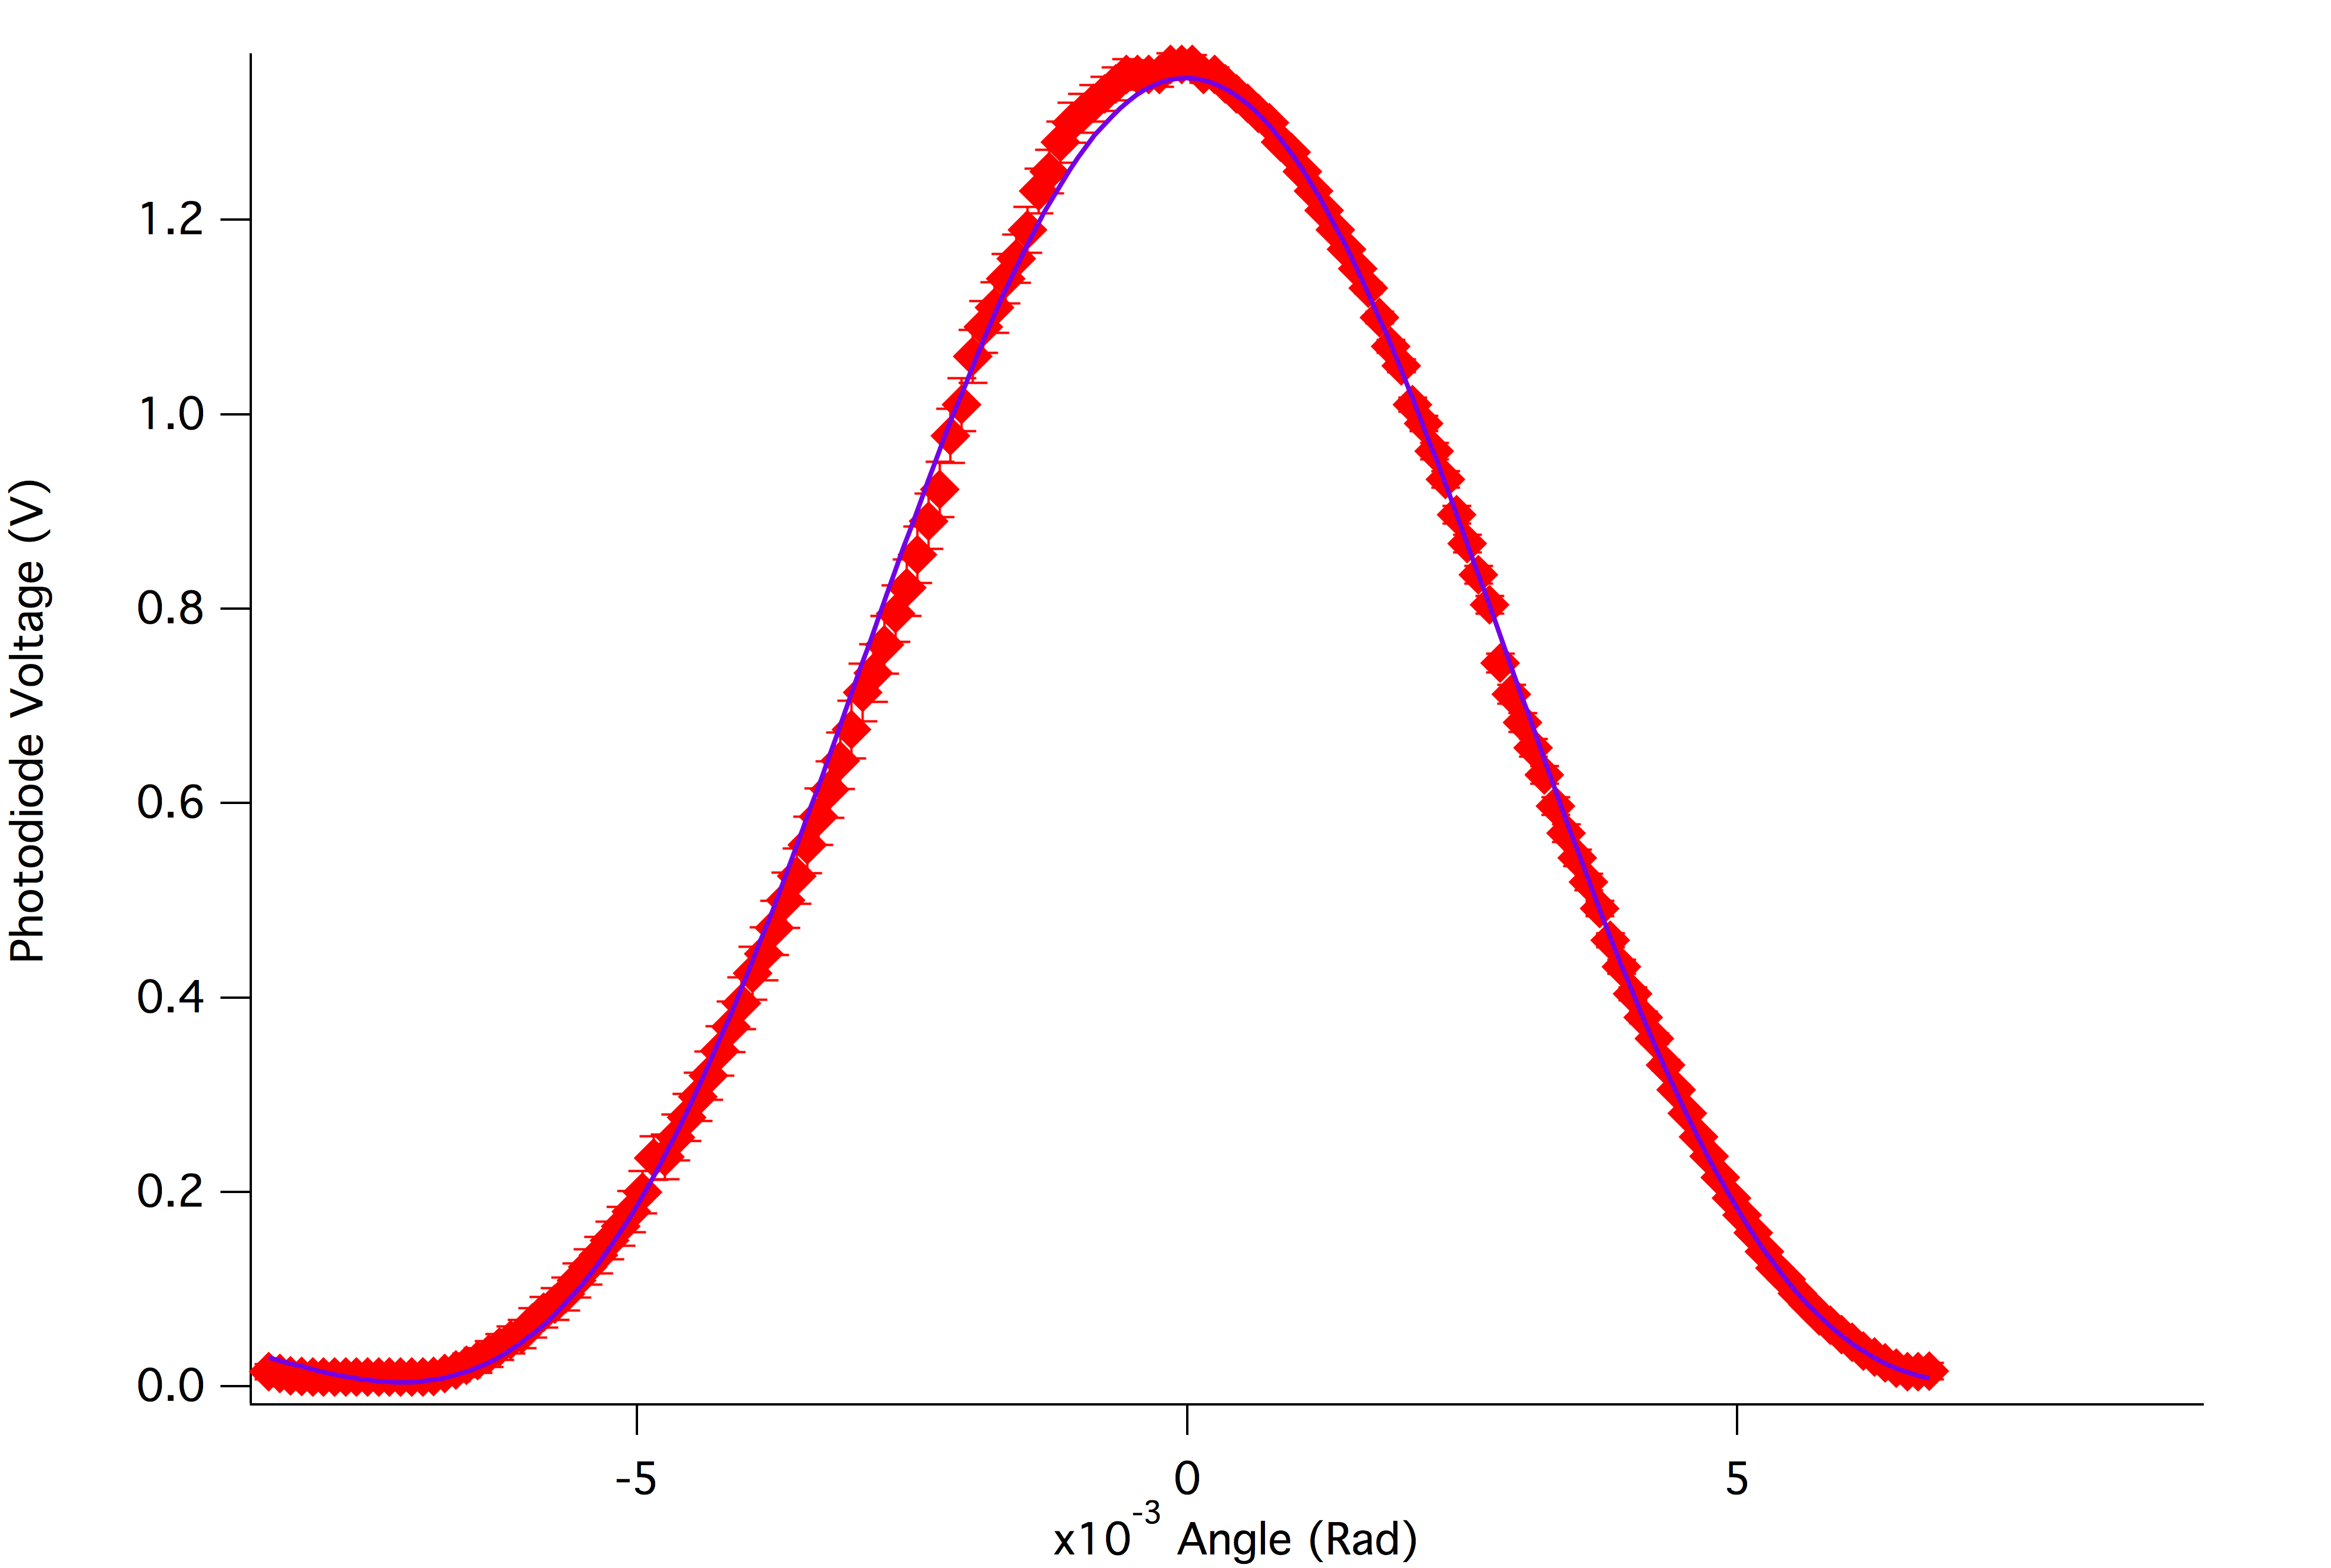
\includegraphics[width=6.6in]{single.png}
\caption{Plot of raw data, error bars and fit curve of the single-slit experiment. The y-axis is still the output voltage of the photodiode, and the x-axis is the angle away from the central maximum.}
\label{single}
\end{figure}

Using plotting tools in Igor while applying Eq.\ref{eq2}, we can obtain the plot shown in Fig.\ref{single}. Calculation of the error bars will be once again included in the discussion section for the single slit experiment.

\begin{table}[h]
\centering
\caption{Single-slit data (The definition for the two offsets will be introduced in Eq.\ref{fitdouble})}
\begin{ruledtabular}
\begin{tabular}{ l c c c}
Name & Symbol & Value & Uncertainties($\pm$)\\
\hline
Slit width & a & 93.9 $\mu m$ & 0.2 $\mu m$\\
Wavelength & $\lambda$ & 0.67 nm & N/A \\
Max voltage & $V_0$ & 1.350 V & 0.002 V\\
Voltage offset & $V_{offset}$ &  0.004 V & 0.001 V\\
Theta offset &$ \theta_{offset}$ & 1E-05 rad & 7E-06 rad \\

\hline
Chi Squared & $\chi^2$ & 1.56815 &
\end{tabular}
\end{ruledtabular}
\label{data}
\end{table}

%____________Discussion____________________________________________
\section{Discussion}

\subsection{Double-Slit Experiment}

The Fraunhofer/Fresnel theory (Eq.\ref{eq1}) of interference gives the intensity of light as a function of angle. The photodiode we use to conduct the experiment outputs a voltage proportional to the intensity of light detected ($I = kV$), thus the intensity measurements can be replaced by the voltage readings and the analysis holds for both:

\begin{equation}
V=V_0 sinc^2( \frac{\pi a}{\lambda} sin (\theta+\theta_{offset}))  cos^2(\frac{\pi d}{\lambda} sin (\theta+\theta_{offset}) + V_{offset}
\label{fitdouble}
\end{equation}

Several parameters are added to the original Fraunhofer model. $V_{offset}$ is describing the affect of the background light. Although the photodiode is kept in a closed black box, there is a slight amount of background light, which will produce an offset and shift the whole curve up. $\theta_{offset}$ describes the systematic error in angle, which is a result of the systematic error in position.\\

Some other parameters need fitting are slit width and slit separation. Due to manufacturing imperfection, the slit width and slit separation have slightly different values than given by the experiment manual. The wavelength of the laser might also be slightly off, but because equation m contains ratio terms $\frac{\pi a}{\lambda}$ and $\frac{\pi d}{\lambda}$, the numerator and denominator cannot change at the same time. Compared to a and d, $\lambda$ is less likely to have a greatly different value, so it is held at 0.67 $\mu m$. $V_{0}$ stands for the voltage measured at the central maximum.\\

Uncertainty in the variable (angle $\theta$) is determined by applying error propagation. Each step of the detector-slit change is designed to be 0.05 mm on the micrometer, from $x_i = 0.15 mm$ to $x_f = 8.35 mm$. Angle $\theta$ corresponds to the position in radian (Fig. \ref{interference}) is given by
\begin{equation}
\theta = \frac{arctan(x-x_0)}{L}
\label{theta}
\end{equation}
$L$ is the distance from the double-slit to the photodiode, is 50 cm given by the experiment manual.
$x_0$ is found to be $4.4 \pm 0.1mm$ given by the Gaussian curve fit to the data set.

\begin{figure}[h]
\centering
\includegraphics[width=7in]{doublegaus.pdf}
\caption{Gaussian curve fit of double-slit interference is made to find the position where the intensity/output voltage of the photodiode peaks.}
\label{gasfit}
\end{figure}
\textcolor{blue}{I suggest using L instead of D, to avoid confusion with d}

However, due to human error \textcolor{red}{in place of the vague and unhelpful term``human error'' explain precisely what source of the error, such as ``due to my lab partner hugging me each time I tried to advance the micrometer'' or ''the precision of the micrometer is limited to 0.025 mm'' or ``since we can only set the micrometer position with a precision of 0.025 mm'' or similar} , each step is not perfectly $0.05 mm$, but $0.05\pm0.03 mm$.
Then the error in angle is given by taking derivative of Eq. \ref{theta} and multiply $\theta^\prime$ by $\delta x$, which is $0.03 mm$. 

\begin{equation}
\theta^\prime = \frac{1}{L(1+(x-x_0)^2)}
\label{thetaprime}
\end{equation}

\begin{equation}
\delta\theta = \theta^\prime \delta x = \frac{\delta x}{L(1+(x-x_0)^2)}
\label{deltatheta}
\end{equation}

$\delta\theta$ is a function of position x. The same method of taking derivative could be applied to find the error in voltage, but it is rather messy. So a different approach is adopted to find $\delta V$, which is to change $\theta$ in Eq. \ref{fitdouble} by $\delta\theta$ and calculate the resulting change in V, which is then divided by 2.

\begin{equation}
\delta V = \frac{\left| V(\theta+\delta\theta)-V(\theta-\delta\theta)\right |}{2}
\label{deltav}
\end{equation}

It can be seen that the same $\delta\theta$ has a smaller impact on $\delta V$ when $V^\prime$ is small, and a bigger impact when $V^\prime$ is big.\\

The multimeter itself also contributes to the error in angle. We estimate the error in meter readings to be $0.05v$.
So the overall $\delta V$ is
\begin{equation}
\delta V_{total} = \delta V+\delta V_{meter} = \delta V + 0.05v
\label{deltavtotal}
\end{equation}
$\delta V$ is plotted as a function of angle in Fig. \ref{double}.\\

The reduced $\chi^2$ is calculated for the fit curve, yielding a value of 0.827. The value is close to 1, meaning that the fit is good within estimation of error. \textcolor{blue}{and, more importantly, your results are well described by the Fraunhofer model for ? slit diffraction}. \\

\subsection{Single-Slit Experiment}

The intensity of light as a function of $\theta$ in single-slit experiment is given by the Fraunhofer/Fresnel theory in Eq. \ref{eq2}, which can then be transformed as
\begin{equation}
V=V_0 cos^2(\frac{\pi d}{\lambda} sin (\theta+\theta_{offset})) + V_{offset}
\label{fitsingle}
\end{equation}
Parameters need fitting are slit width $(a)$, slit separation $(d)$, maximal voltage $(V_0)$, offset in voltage $(V_{offset})$ due to background light, and offset in $\theta$ $(\theta_{offset})$ due to systematic error of position.\\

Uncertainty is determined using the same method. $\theta$ is found using Eq. \ref{theta} while x goes from $x_i = 0.15mm$ to $x_f = 7.7mm$ with a step size of $0.05mm$. However, the value of $x_0$ need re-calculating, since the single-slit pattern is slightly shifted than the double-slit pattern. A Gaussian fit is done to the data to determine $x_{offset}$, which is $4.327 \pm 0.003mm$.\\

\begin{figure}[h]
\centering
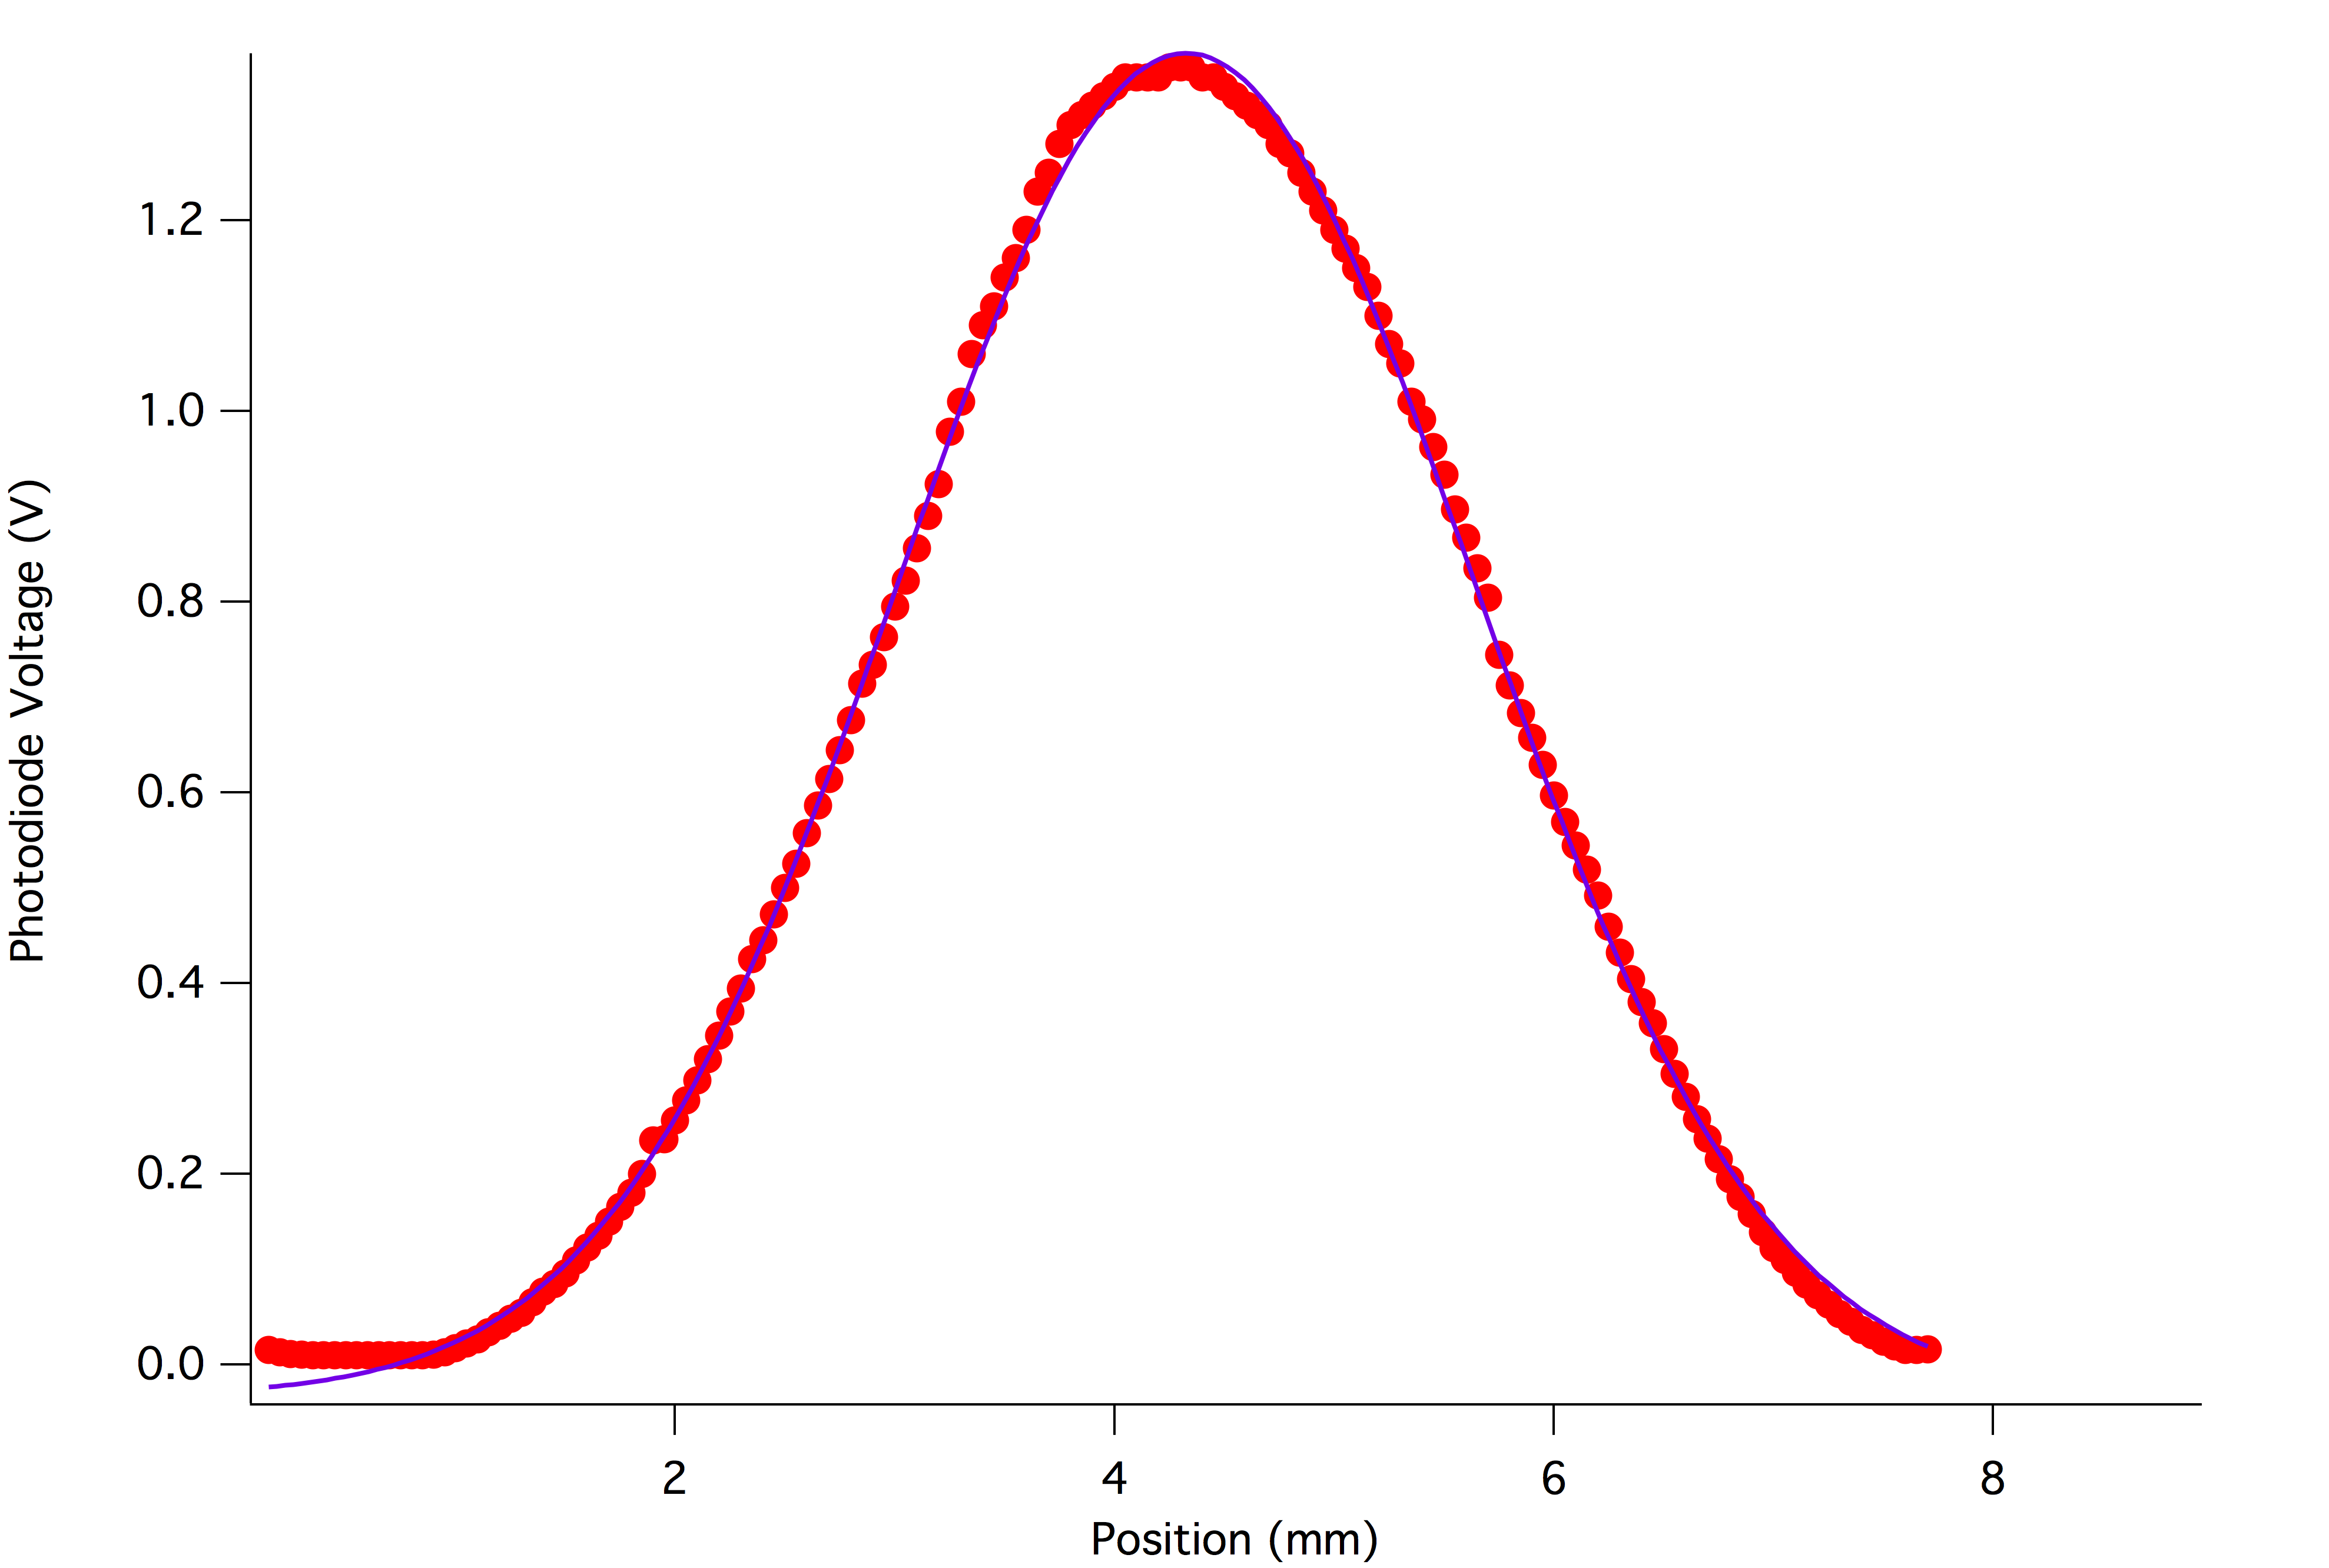
\includegraphics[width=7in]{singlegaus.png}
\caption{Gaussian curve fit of single-slit diffraction is made to find the position where intensity/output voltage of the photodiode peaks.}
\label{gasfit2}
\end{figure}

The slit to detector distance L remains $50 cm$. Uncertainty in step size is also considered to be $0.03mm$, as in the double-slit experiment. Eq. \ref{thetaprime}, \ref{deltatheta} and \ref{deltav} are used to determine uncertainty in voltage. In the final step of calculating $\delta V_{total}$ (Eq. \ref{deltavtotal}), $\delta V_{meter}$ is changed to $0.01v$, because the single-slit pattern has smaller intensity and thus a fluctuation of smaller scale in voltage.

The reduced $\chi^2$ is 1.56815, which is approximately 1, showing the fit is good within our estimate of error. \textcolor{blue}{not quite, but close. what is the probability that the model fits the data, if the reduced chi-square has a value of 1.6? Answer: if 6 or 7 degrees of freedom, then somewhere between 10 and 20 percent. See squires or http://www.pd.infn.it/~lunardon/didattica/docsper2/TavoleChi2.pdf , for example. You can see that there is a systematic error in Fig 8 between fit and data as position approaches zero and that the measured peak is slightly assymmetrical, perhaps because the traveling slit in front of the detector is slightly tilted?}. 

\subsection{Comparison}

Looking at parts A and B, we see that the the maximum voltage ($V_0$) for the double-slit is approximately 4 times the maximum voltage for the single-slit equation. This is because when two central maximums of the two slits are superposed, the amplitude doubles at the central maximum ($\theta = 0$). The intensity is proportional to the amplitude squared: $$I \propto A^2 \ \ \ \	4I \propto(2A)^2$$ This relationship is clearly shown in our experiment: $$\frac{V_{0,double}}{V_{0,single}}=\frac{A_{0,double}^2}{A_{0,single}^2} = \frac{4.55\pm 0.07}{1.350 \pm 0.002}=3.37 \pm 0.06 \approx4$$ As we can see, the Voltage  double slit quadrupled.

\textcolor{red}{I don't think you can claim that a ratio of 3.37 clearly demonstrates that the signal quadrupled.  Perhaps the photodiode response is starting to saturate at high intensities, and is no longer linear near the central peak of the two-slit pattern? Perhaps the traveling slit in front of the detector is slightly tilted, and therefore smooths out and (lowers the max value) of the peaks? What you can definitely claim, however, is that you have shown that due to wave inteference, the combined waves have a maximum intensity that is greater than that which would be expected in the absence of wave interference. That is, 3.37 is significantly greater than 1 + 1, even if it is less than 4. } 




%____________Conclusion____________________________________________
\section{Conclusion}

 The observed interference pattern is fitted using Fraunhofer model, which describes far-field diffraction. The amplitude of the double-slit pattern was observed to be the modulated by the single slit diffraction pattern. Reduced $\chi^2$ of the double-slit fit curve is 0.827 and that of the single-slit fit curve is 1.57.

\textcolor{blue}{need something here about how this demonstrates that light behaves as a wave (diffracting and interfering) rather than as a ray, as first demonstrated by Young} 


\begin{acknowledgments}

We gratefully acknowledge \textcolor{magenta}{Nathaneal} Fortune and Dana Parsons, who helped with the experimentation and editing of this experiment.  This work was supported by the Smith College Physics Department.

\end{acknowledgments}


\begin{thebibliography}{99}

\bibitem{wik} Double Slit Experiment, \url{<http://upload.wikimedia.org/wikipedia/commons/c/c2/Single_slit_and_double_slit2.jpg
/>}.

\bibitem{dia} TeachSpin Instructions Manual,\textit{Two-Slit interference, One Photon at a Time (TWS1-B), Pulse Counter/Interval Timer (PCIT1)}, 6/2013.
\bibitem{interference} Young Two-Slit Experiment, \url{http://abyss.uoregon.edu/~js/21st_century_science/lectures/lec13.html}

\end{thebibliography}

%\newpage   % Start a new page for tables

\end{document}
